\chapter{Performance Test}

As with many network protocols designed to transfer data quickly and reliably, there needs to be performance analysis. The performance of MCDTP is measured by throughput and packet loss.

\section{Test Environment}

The test environment used to test MCDTPi used commodity servers rented from a cloud computing company called DigitalOcean. Two servers were rented, one deployed in New York, USA and the second deployed in Amsterdam, Netherlands---the distance was deliberate to test MCDTPi over WAN. The rented servers were configured with 4 CPUs, 8GB of RAM, 80GB SSD, and 5TB of transfer and run Ubuntu 16.04LTS. DigitalOcean does not disclose any server specifications beyond this. The servers were further configured with the cross-platform version of .NET Framework, .NET Core 1.0.3, in order to execute the tests for MCDTPi.

The Ethernet link of both servers places a constraint on the size of transmitted packets. This constraint is know as the Maximum Transmission Unit (MTU). The MTU for both servers was 1500 bytes. The largest a packet can be is 1500 bytes before it gets fragmented into smaller packets. Fragmentation is not handled by MCDTP, so MCDTPi was compiled with a UDP packet size set to 1400 bytes to account for any packet headers.

\section{Testing}

There were four test configurations applied to MCDTPi. All configurations used a 1GB file as the data source. Since both servers had 8GB of main memory, for each test, MCDTPi was able to hold the entire file in memory. Thus disk I/O was not a factor in performance. The variable between each test was the number of channels MCDTPi used on each test---single-, dual-, quad-, and octa-channel configurations.

Since throughput and packet loss are used as performance measurements, only the Data Transmission phase of MCDTP is tested. This is to test the unreliability of MCDTP. By measuring unreliability, it gives insight as to how much work would need to be done to provide reliability.

\subsection{Test Results}

For the following tests, the server in New York played the role of client and the Amsterdam server played the role of server, which was arbitrarily decided since exact specifications on the servers are unknown and thus could not weigh in on this.

Figures \ref{fig:tr-ct} and \ref{fig:tr-st} show the throughput in bytes for single-, dual-, and quad-channel configurations for both client and server hosts, respectively. These results are discussed in section \ref{sec:anlys}.

Tables \ref{tab:server-perf} and \ref{tab:client-perf} show further statistics on performance. Figures \ref{fig:tr-at}, \ref{fig:tr-mt}, and \ref{fig:tr-pl} are the graphical representation of this data. These results are discussed in section \ref{sec:anlys}.

\begin{table}[H]
\centering
\caption{Server Performance}
\label{tab:server-perf}
\begin{tabular}{rcccc}
\multicolumn{1}{c}{} & Single    & Dual      & Quad       & Octa  \\
Average Throughput   & 1.146Mbps & 2.893Mbps & 0.545Mbps  & 0Mbps \\
Max Throughput       & 4.385Mbps & 6.998Mbps & 12.065Mpbs & 0Mbps \\
Packet Loss          & 14.06\%   & 19.64\%   & 87.97\%    & 100\%
\end{tabular}
\end{table}

\begin{table}[H]
\centering
\caption{Client Performance}
\label{tab:client-perf}
\begin{tabular}{rcccc}
\multicolumn{1}{c}{} & Single    & Dual      & Quad       & Octa  \\
Average Throughput   & 1.018Mbps & 2.398Mbps & 0.52Mbps  & 0Mbps \\
Max Throughput       & 3.879Mbps & 5.934Mbps & 11.755Mpbs & 0Mbps
\end{tabular}
\end{table}


\section{Analysis}\label{sec:anlys}

The expected behavior of MCDTPi is that as resources increase with more channels, throughput and packet loss improve. The test results show that this behavior is partly true going from single-channel to dual-channel. Throughput improved two fold while packet loss had marginal degradation. However, performance worsened in both measurements for quad- and octa-channel configurations. Octa-channel was omitted in Figures \ref{fig:tr-ct} and \ref{fig:tr-st} because tests stalled and yielded no data. Though the Figure \ref{fig:tr-mt} shows quad-channel achieving the highest throughput, it had an average throughput that was half that of the single-channel. Quad-channel had over 6 times as much packet loss as well. This is all around worse.

This outcome seems counter intuitive to what is expected. Nonetheless, this can be explained. To start, the single-channel itself is severely under-perfomant compared to other protocols like RBUDP and Tsunami. Those protocols achieve 300-500 times as much throughput compared to MCDTP. The major difference between this project and those is that MCDTPi experiments with using asynchrony to enhance performance.

The TPL library is the foundation for asynchrony in the .NET Framework \cite{Leijen2009}. As discussed in this blog \cite{Lippert}, the TPL can bog down the performance of a program if too many tasks are created. The TPL library may provide lightweight task management, especially when compared to multi-threading; however, to manage numerous tasks begins to add overhead thus impacting performance.

The granularity of asynchrony in MCDTPi is at the packet level. This means that for every packet, there is an asynchronous task. For these tests, there are nearly 800,000 asynchronous tasks created to handle only sending packets. The lifespan of a packet requires two more asynchronous task on a single host. This means that for a single file transfer 2.4 million tasks are created, causing significant overhead.

Single-channel and dual-channel were able to operate since the number of scheduled asynchronous tasks was more spead out. Quad-channel and octa-channel scheduled tasks more rapidly and either caused very low throughput, or a complete halt to the program.

\newpage

\begin{figure}[ht]
\centering
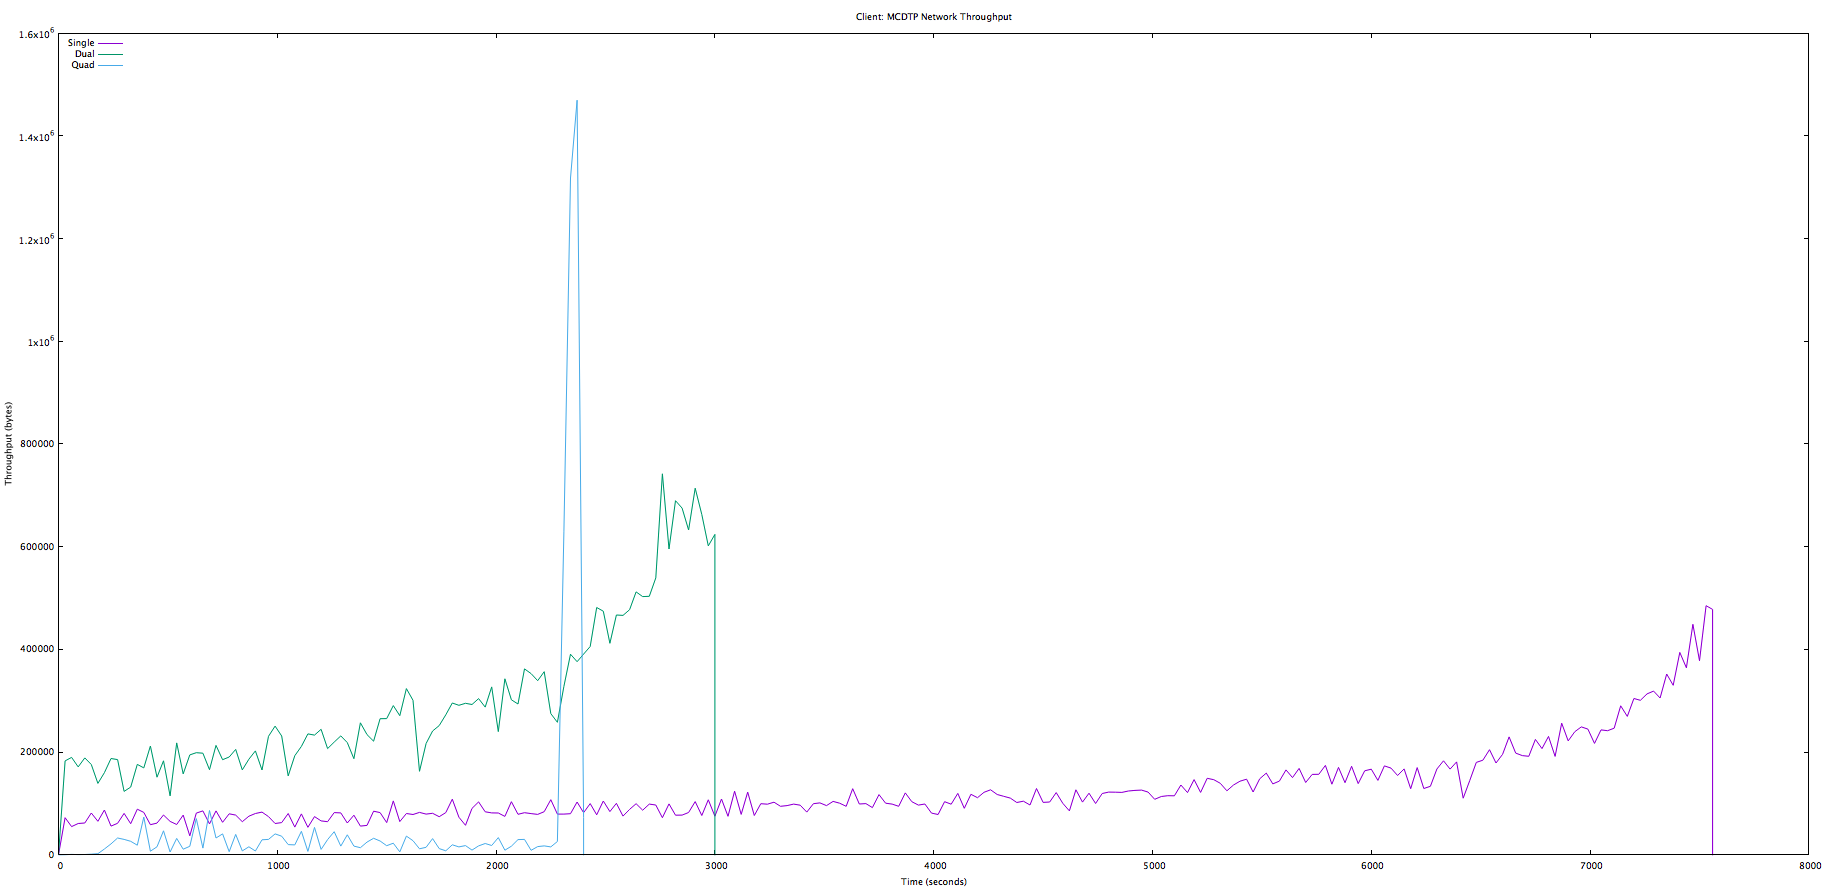
\includegraphics[scale=0.4]{TestResultClientThroughput}
\caption{Client Throughput}
\label{fig:tr-ct}
\end{figure}

\begin{figure}[ht]
\centering
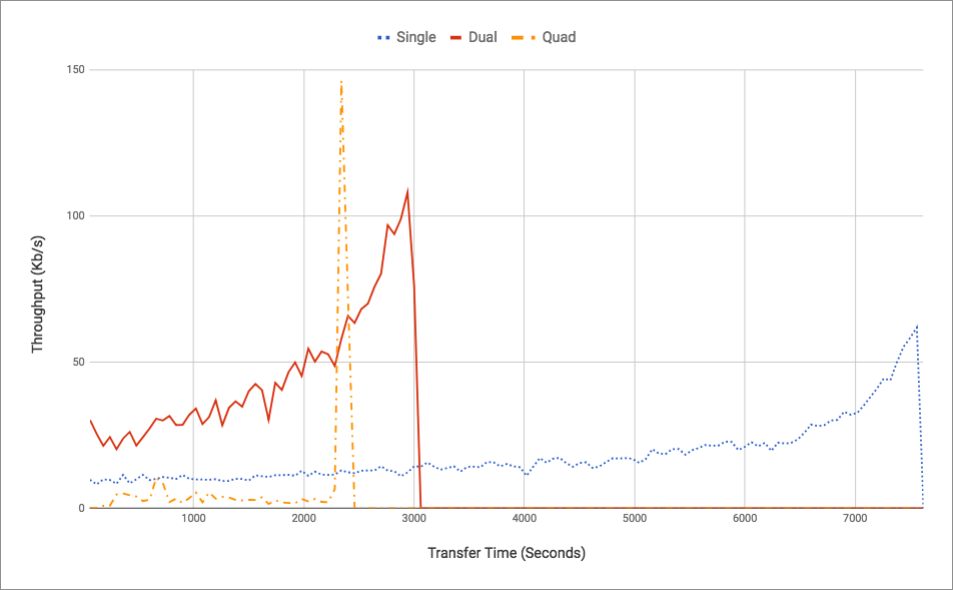
\includegraphics[scale=0.4]{TestResultServerThroughput}
\caption{Server Throughput}
\label{fig:tr-st}
\end{figure}

\begin{figure}[ht]
\centering
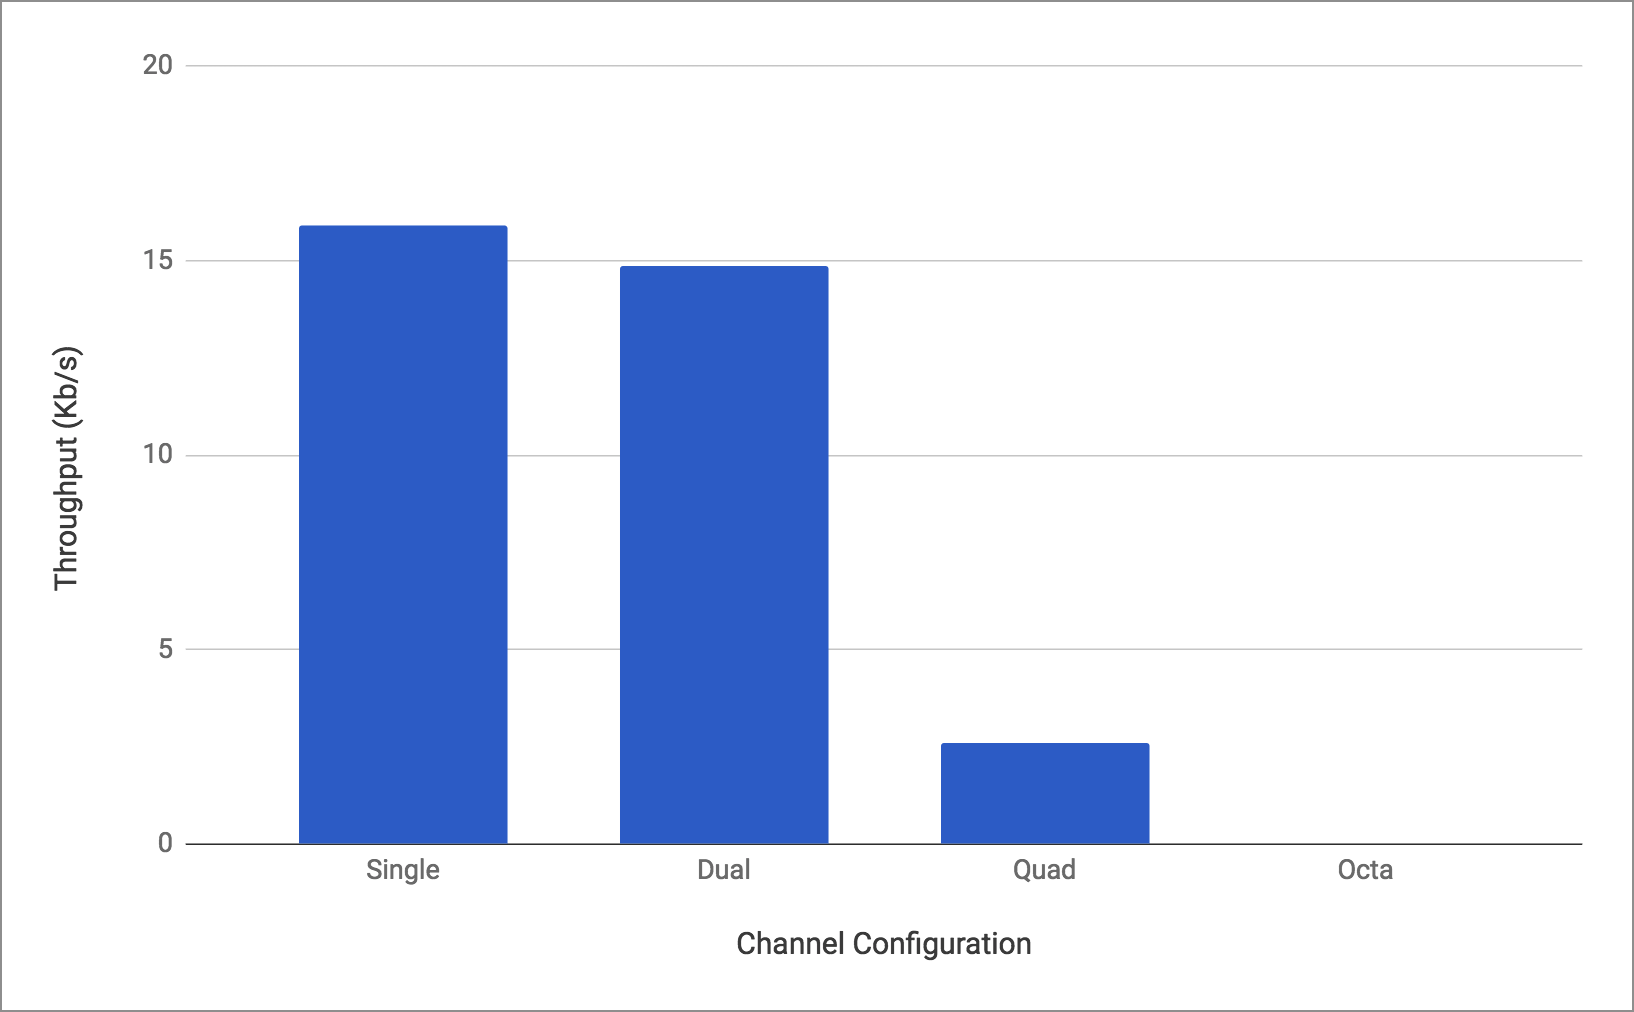
\includegraphics[scale=0.4]{TestResultAverageThroughput}
\caption{Average Throughput}
\label{fig:tr-at}
\end{figure}

\begin{figure}[ht]
\centering
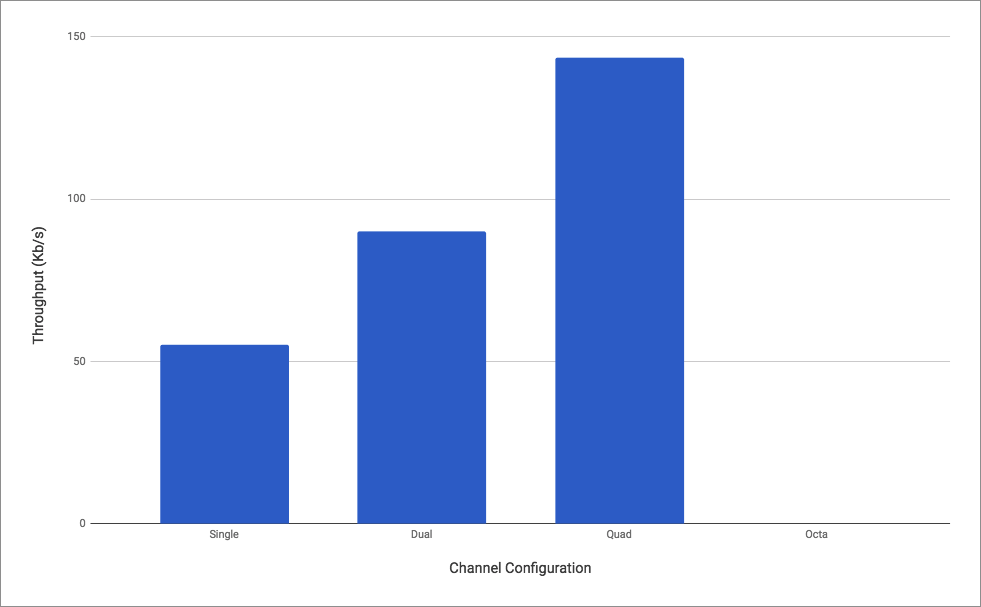
\includegraphics[scale=0.4]{TestResultMaxThroughput}
\caption{Max Throughput}
\label{fig:tr-mt}
\end{figure}

\begin{figure}[ht]
\centering
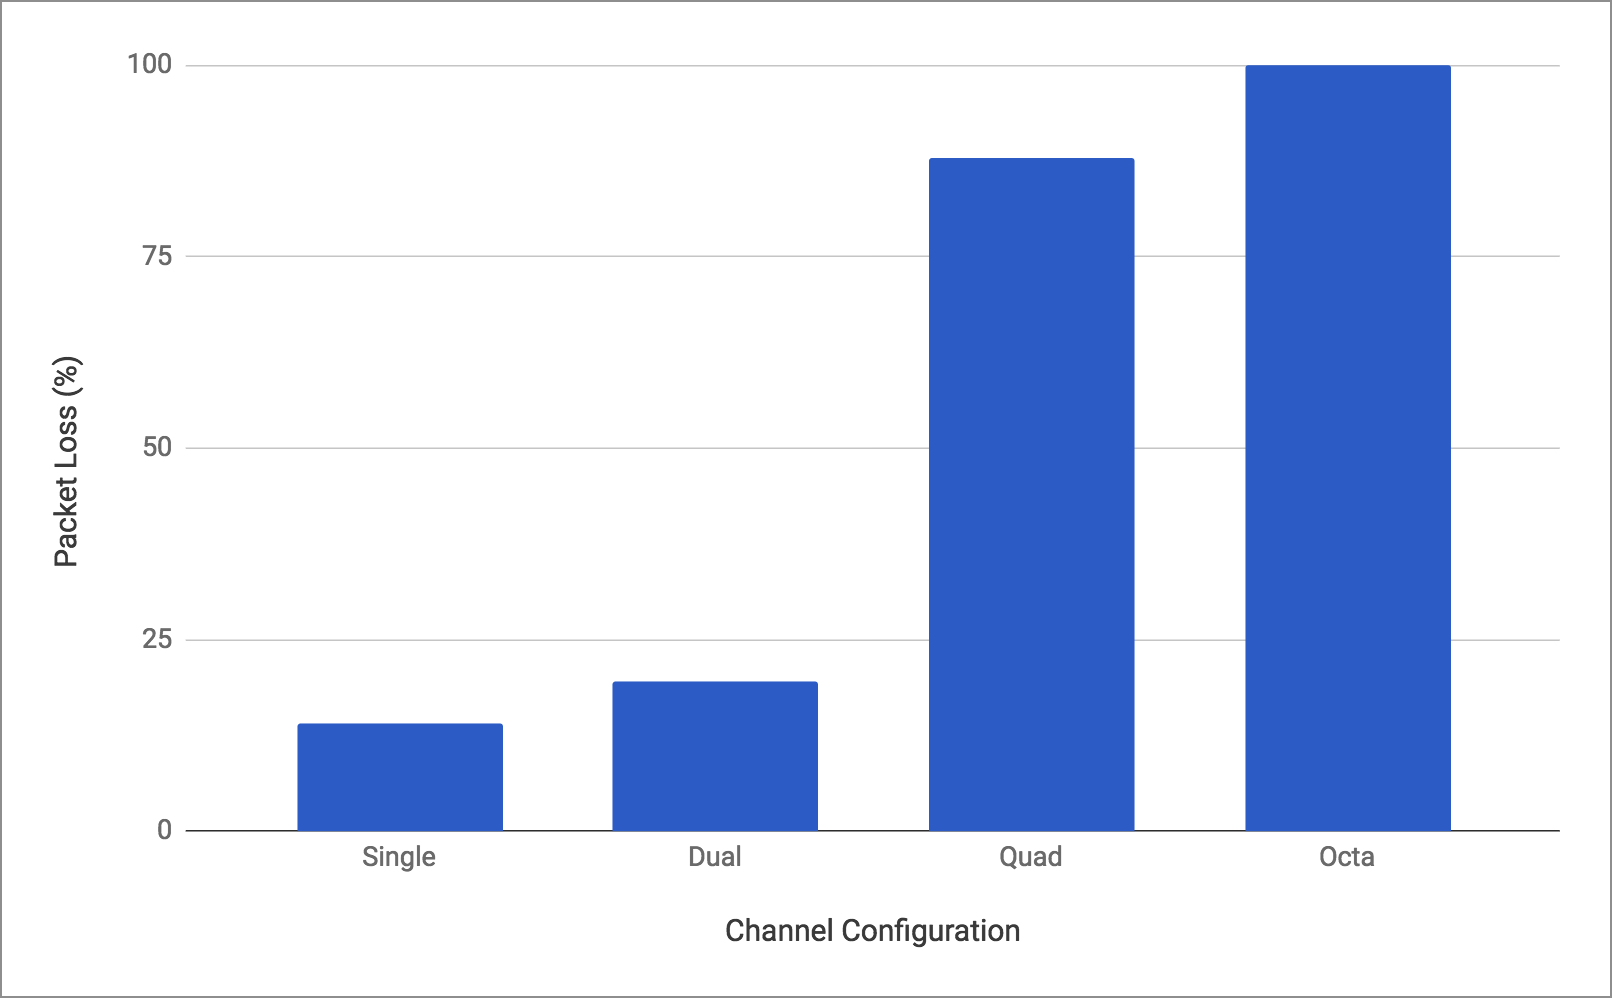
\includegraphics[scale=0.4]{TestResultPacketLoss}
\caption{Packet Loss}
\label{fig:tr-pl}
\end{figure}